\documentclass[11pt]{article}
\usepackage{lscape}
\usepackage[table]{xcolor}% http://ctan.org/pkg/xcolor
\setlength{\parindent}{0pt}
\usepackage [colon]{natbib}
\usepackage {comment}
\renewcommand{\familydefault}{\sfdefault}
\usepackage[a4paper, margin=2.40cm]{geometry}
\usepackage{doi}
\usepackage{multirow}
\usepackage[T1, OT1]{fontenc}
\DeclareTextSymbolDefault{\dh}{T1}
\renewcommand{\rmdefault}{phv} % Arial
\renewcommand{\sfdefault}{phv} % Arial
\usepackage[modulo]{lineno}
\usepackage{wrapfig}
% \linenumbers
\usepackage{hyperref}
\usepackage{array}
\newcolumntype{L}[1]{>{\raggedright\let\newline\\\arraybackslash\hspace{0pt}}m{#1}}
\newcolumntype{C}[1]{>{\centering\let\newline\\\arraybackslash\hspace{0pt}}m{#1}}
\newcolumntype{R}[1]{>{\raggedleft\let\newline\\\arraybackslash\hspace{0pt}}m{#1}}
\usepackage{amsmath}
\usepackage{float}
% \errorcontextlines=3
\usepackage[explicit]{titlesec}
\usepackage{graphicx}
\usepackage{caption}
\usepackage{authblk}
\usepackage{setspace}
\usepackage[export]{adjustbox}
\renewcommand{\bibfont}{\footnotesize}
\usepackage{bibentry}
\usepackage{tikz}
\usepackage[inline,shortlabels]{enumitem}
\usepackage[all]{nowidow}


\newcommand{\alpine}{\textit{ALPINE}\,}
\newcommand{\icesheet}{\textit{ICESHEET}\,}
\newcommand{\TODO}[1]{\textbf{TODO #1}}
\newcommand{\ian}[1]{{\textbf{\color{blue}Ian says:} \color{blue} #1} }
\newcommand{\leif}[1]{{\textbf{\color{red}Leif says:} \color{red} #1} }
\newcommand{\frederic}[1]{{\textbf{\color{red}Frederic says:} \color{red} #1} }
\newcommand{\aref}[1]{\textbf{Reference #1}}
\title{}
\author{}

\begin{document}
Dear Editor,

\vspace{.2cm}

We thank Reviewer 2 for their comments. We believe that in addressing them, we have clarified the model presentation. We note, however, that the presentations of criticisms by the reviewer was at times difficult to respond to, given the format of the review. Please let us know if additional points should be addressed. 

\vspace{.2cm}

The reviewer's comments are in bold, our response is in italics and quotations from the new text are in normal font.

\vspace{.2cm}

Best regards,

\vspace{.75cm}

Ian Delaney on behalf of all authors

\vspace{2cm}

\textbf{General Comments}

\begin{itemize}

\item \textbf{
    The trouble is, that while the first term on the right hand side of (3) makes sense to me, the second does not, and the reason for this is that the closure term involves the effective pressure and thus the hydraulic head, but not its gradient, so I am a bit sceptical about this, because the structure of the Nye model seems to have been altered.
    You might say that the distinction disappears in the lumping, but it seems to me that if you have an upstream head h- and a downstream head h+, the first term on the right of (3) will involve the difference, but the second will involve the average, and there are two independent quantities involved.
    I suppose you can get around this by saying, oh, the outlet head or more accurately the effective pressure is zero, and perhaps that is what is done.
    But that is a bit disingenuous, because the outflow becomes open channel flow somewhere upstream of the actual mouth of the stream.
    Now I went and looked up this Werder 2010 paper, and you can see in its equation (4) the same distinction I am making here.
    I suppose my overall view is that (I think) the Clarke paper intended to use the flow elements of resistors, etc., as ingredients of a larger scale flow path, and this lumping of a whole channel is an extremely coarse thing to do, and looks a bit like avoiding confronting the spatially-dependent physics simply because it’s too hard.
    So I think you can rescue this aspect of the model presentation, but a bit more exposition would help, in particular the figure 2or equivalent of the 2010 paper would help.}


  \textit{We thank the reviewer for this comment, as it demands clarification in our model presentation. To reduce the number of variables in the original text, $h_p$ was omitted as its value is zero, as is the hydraulic head at the glacier terminus. The text has been updated to clarify this point.
    Additionally, we confirm the reviewer's comment, that effective pressure at the glacier terminus is zero. The text will read:}
  The evolution of subglacial channel size $S_g$ is given as
  \begin{linenomath*}
    \begin{equation}
      \label{eq:dS_dt}
      \frac{\partial S_g}{\partial t} = C_1 \frac{Q \Delta h}{l} - C_2 \left(h_{o}-\overline{h}\right)^n\,S_g,
    \end{equation}
  \end{linenomath*}
  \noindent where $t$ is time, $C_1= (1-\rho_wc_pc_t)\,\frac{\rho_wg}{\rho_iL}$ and $C_2=2A(\frac{\rho_wg}{n})^n$ are constants (values in Table~1), $g$ is the acceleration due to gravity, $Q$ is water discharge, $\overline{h}=\frac{1}{2}(h+h_p)$ is the mean hydraulic head in the channel with $h_p$ being the proglacial hydraulic head equal to zero, $l$, $h_{o}= \frac{\rho_i}{\rho_w} h_{ice}$ is the mean ice overburden pressure expressed in meter water equivalent ($\rho_w$ is density of water; $\rho_i$ is density of ice), and $n$ is Glen's n \citep[usually $n=3$; ][]{glen1955}.
  The first term on the equation's right side represents the channel opening by frictional heating, while the following term represents channel closure from ice deformation.


  \textit{
    The reviewer also correctly points out that water de-pressurizes underneath the glacier, in agreement with the other reviewer, we have included a comment that we assume pressurized flow across the glacier bed, as is common in subglacial hydrology models, although this may not always be the case \citep{perolo2018}.
  }
  
  \textit{Lastly, we have chosen a simple model, lumped element, or channel segment model here as we believe that it most clearly and concisely explains the dynamics that we wish to discuss.
    Our strong opinion is that the experiments that we have done with the model, across a range of hydrographs, demonstrate consistently the behavior of subglacial channels.
    Therefore, we do not believe that a more complex model is needed to show these processes.
    The limitation of this approach is acknowledged and discussed.
  }

\item  \textbf{And the model should come with some caveats, e. g., you could say that it is a simplistic and possibly unreliable model. To be fair, this is done in section 5.3, but that is too late.}

  \textit{The ``Methods'' section is largely meant to describe the model, as opposed to discussing its behavior or simplicity. In response to this comment, we will move the ``Experiment limitations'' to a section directly after the ``Results'' but before the ``Discussion.''}

  
\item \textbf{  One of the comments made is that because the sub-aerial model has an algebraic relation between width and discharge (equation 9), the relationship between velocity and discharge is also algebraic; but this is simply a choice of the model. In reality, the width of a channel will also evolve over (long) time through processes of bank erosion, and the use of equation 9 properly only involves a long term time average of discharge, so it is misleading to use it in a time-specific way. Actually, this is admitted at line 370, along with other limitations in the models.}


  \textit{We appreciate these comments. With regard to the first point about channel width evolution in the subaerial model, this matter is confronted in Sections 4.2 and 4.3 (now 5.1).
    Here we show that across a range of exponents and relationships between channel cross-section and water discharge, subglacial systems are still more sensitive to water discharge variations than subaerial ones.
    This increased variability occurs across a range of $\alpha$ values that describe the relationship between channel width and water discharge as shown in Figure 6 (now 7).
    As a result, we believe that these results hold across a range of water discharge- channel width relationships, including ones where $\alpha$ evolves in time.
    The exception, shown in Section 4.3 (now 6.1), is that when water discharge evolves more slowly than channel size. Here, the behavior between subaerial and subglacial is very similar, because channel areas in both channel types adjust to discharge variations.}
  

\item   \textbf{Two kinds of numerical experiments are described in section 3.3, and the results of these presented in section 4. Presumably the input to the model runs is the (time- varying) water discharge, but that seems not to be stated in 3.3, which I would expect, although it is stated in the caption to figure 2.
    The second half of the paper characterises the results of these experiments and there is an extended discussion. There is no doubt the authors have put a lot of effort into this, but my interest waned at this point.}
 
  \textit{To make it clear that water discharge is the input, we will modify the first sentence of Section 3.3 to explicitly state:}
    ``Proglacial discharge records from the Fieschergletscher (scenario \alpine{}) and the Leverett Glacier (scenario \icesheet{}) are used as inputs for the models above.''

\item \textbf{  In summary, this is one of those difficult papers to judge, because the effort in- volved is quite substantial and honestly applied, but the whole philosophy of the approach is, in my view, misguided. This is a coxless boat crew who are rowing up a backwater without a rudder, and have lost the main direction of the stream.}

  \textit{With respect to the last sentence, it is true that the lead author feels this way occasionally. Regardless, we think valuable findings are within this manuscript.}

\end{itemize}

\textbf{Specific Comments}

\begin{itemize}
\item \textbf{33: I don’t know what ‘Following mass conservation’ has to do with this.}

  \textit{We will remove this phrase.}
  
\item \textbf{99-100: upon that of Clarke.}

  \textit{Done.}

\item \textbf{102: presumably $h_{ice}$ is the thickness of the ice, but the syntax is not clear, it could be the depth of the channel.}

  \textit{The text will read:} `` a glacier with channel length $l$, with a flat bed and a mean ice thickness of $h_{ice}$.''
  
\item \textbf{eq. 3: it’s probably in the Werder 2010 paper, but I’d like to see an extra comment about where this $\frac{\Delta h}{2}$ term comes from.
  Since the bracket represents $N = pi-pw$, $pw$ the pointwise form of this second term would be $\frac{p_w}{\rho_wg}$, so it’s not obvious to me where the $\Delta h$ comes from.
  Also in this light, it is worth elaborating the confusing term ‘hydraulic head drop change’ and defining what $\Delta h$ is in terms of $pw$.
  Actually, the more I think about this, the more suspicious I become. And in fact, at least when you’re dealing with j\"okulhlaups, the discharge doesn’t vary much along the length of the channel, and the consequence of that is that neither does the effective pressure.
  Of course, that may not apply here but I think the same principle applies.
  So maybe I am promoting this to a more substantive issue
  (as indeed now further discussed earlier).}

  \textit{The comment about $\frac{\Delta h}{2}$ is addressed above. We understand the point about flow accumulation and increasing water discharge along the channel. As the author points out, the implications of this are presented in the ``Experiment limitations.'' Additionally, we note that despite these effects, the results here show convincingly that the main topics in the paper still hold, i.e. sediment transport capacity is more variable in subglacial channels than subaerial ones and sediment transport capacity does not vary with water discharge if the subglacial channel size is out of equilibrium with water discharge. }


\item \textbf{114:} I had no idea what the central angle referred to, but evidently it is the angle subtended at the centre of the circular arc of the channel upper boundary; and then $\beta = 2\alpha$, where $\alpha$ is the contact angle at the channel edge, which seems a more natural quantity to use. Also I checked the algebra of equation (5), and got this formula, but with the factor of two in the numerator, not the denominator, assuming hydraulic diameter is twice hydraulic radius, the latter of which is area/perimeter, so please check this. Incidentally, I did also then check equation (7) and I agree with that, so I do think there is an error in (5).

  \textit{We thank the reviewer for the careful assessment of our work. We have double-checked and believe that there is no problem in the equation. Our proof is below:}

   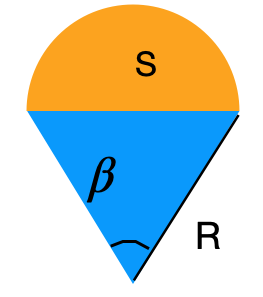
\includegraphics[width=0.3\linewidth]{Hooke.png}
  Guiding equations:

  \begin{equation}
    D_h = \frac{4S_g}{P_w}~~~(I)
  \end{equation}

  \begin{equation}
    P_w = R \beta +2R \sin\frac{\beta}{2}= R(\beta +2\sin \frac{\beta}{2} ~~~(II)
  \end{equation}

  \begin{equation}
    S_g=\frac{R^2}{2}(\beta - \sin \beta)~~~(III)
  \end{equation}

  $D_h$ is hydraulic diameter, $P_w$ is wetter perimeter, $R$ is radius, $\beta$ is Hooke angle \citep{hooke1990}, and $S_g$ is the subglacial channel cross section.

  Proof:
  
  \begin{linenomath*}
    \begin{equation}
      \frac{D_h}{4S_g} = \frac{1}{R\beta + 2R\sin\frac{\beta}{2}}
    \end{equation}
  \end{linenomath*}

  \begin{equation}
    R = \frac{4S_g}{D_h (\beta +2 \sin \frac{\beta}{2})}, \quad \mathrm{into~} III 
  \end{equation}

  
  \begin{equation}
    S_g = \frac{16 S_g^2}{D_h^2 (\beta +2\sin\frac{\beta}{2})^2} ~\frac{1}{2}(\beta-\sin\beta)
  \end{equation}

  
  \begin{equation}
    1 = \frac{8 S_g}{D_h^2 (\beta +2\sin\frac{\beta}{2})^2} (\beta-\sin\beta)
  \end{equation}


  \begin{equation}
    \frac{D_h^2}{8} \frac{(\beta+2\sin\frac{\beta}{2})^2}{\beta - \sin \beta} = S_g
  \end{equation}

  \begin{equation}
    \frac{D_h^2 (2(\frac{\beta}{2}+\sin \frac{\beta}{2}))^2}{8(\beta - \sin \beta)} = S_g
  \end{equation}


   \begin{equation}
    \frac{D_h^2 ((\frac{\beta}{2}+\sin \frac{\beta}{2}))^2}{2(\beta - \sin \beta)} = S_g
  \end{equation}


  \begin{equation}
       S_g = \frac{D_h^2}{2} \frac{(\frac{\beta}{2}+\sin \frac{\beta}{2})^2}{(\beta - \sin \beta)}  
  \end{equation}

  This is the same as Equation 5 of our manuscript.

  

\end{itemize}

\bibliographystyle{apalike} 
\bibliography{../PaperLib.bib}
\end{document}

